\documentclass[tikz,border=2pt]{standalone}
\usepackage{amsmath}
\usepackage[T1]{fontenc}
\usepackage[tt=false, type1=true]{libertine}
\usepackage[varqu]{zi4}
\usepackage[libertine]{newtxmath}
\usetikzlibrary{positioning,arrows.meta,fit,backgrounds,calc}

\newcommand{\Z}{\mathbb{Z}}

\definecolor{ink}{HTML}{16191D}
\definecolor{accent}{HTML}{1F4E79}
\definecolor{accentsoft}{HTML}{E8EEF4}
\definecolor{accentwarm}{HTML}{9A5B00}
\definecolor{accentplum}{HTML}{8E2F5F}
\definecolor{muted}{HTML}{5B6470}
\definecolor{hairline}{HTML}{C9CFD6}

\tikzset{
    house/.style={
    >={Stealth[length=2.1mm, width=1.6mm]},
    line width=0.5pt,
    node distance=9mm and 15mm,
    every node/.style={font=\small},
  },
    box/.style={
    draw=ink, line width=0.5pt, rounded corners=1.5pt,
    inner xsep=6pt, inner ysep=4pt, align=center,
  },
    boxhi/.style={box, draw=accent, fill=accentsoft, text=ink},
    boxdim/.style={box, draw=hairline, text=muted},
    flow/.style={->, draw=ink},
  flowdim/.style={->, draw=hairline},
  lbl/.style={font=\footnotesize\itshape, text=accent, inner sep=2pt},
  lbldim/.style={font=\footnotesize, text=muted, inner sep=2pt},
    group/.style={draw=hairline, dashed, rounded corners=2pt, inner sep=7pt},
}

\definecolor{stateink}{HTML}{006A7B}
\definecolor{certink}{HTML}{6D3D85}

\tikzset{lbldim/.style={font=\small, text=muted, inner sep=2pt}}
\begin{document}
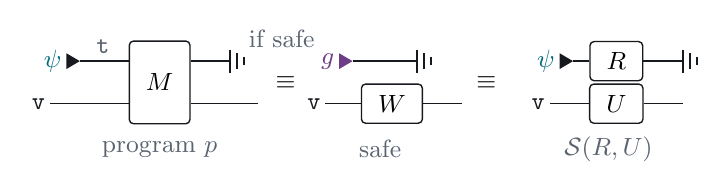
\begin{tikzpicture}[house, semithick, font=\normalsize,
  bx/.style={box, fill=white, minimum width=7.5mm, minimum height=10.5mm},
  sm/.style={box, fill=white, minimum width=6.5mm, minimum height=4.6mm},
  gnd/.pic={\draw[ink] (0,0) -- (0.10,0); \draw[ink] (0.10,0.145) -- (0.10,-0.145);
            \draw[ink] (0.19,0.100) -- (0.19,-0.100); \draw[ink] (0.28,0.055) -- (0.28,-0.055);}]
\node[bx] (U) at (0,0) {$M$};
\coordinate (a1) at ($(U.west)+(-0.62,0.27)$);
\draw[ink] (a1) -- ($(U.west)+(0,0.27)$);
\fill[ink] (a1) ++(-0.17,-0.10) -- ++(0,0.20) -- ++(0.17,-0.10) -- cycle;
\node[left, font=\small, inner sep=1.5pt, text=stateink] at ($(a1)+(-0.17,0)$) {$\psi$};
\draw[ink] ($(U.west)+(0,-0.27)$) -- ++(-1.0,0) node[left, font=\small, inner sep=1.5pt] {\texttt{v}};
\draw[ink] ($(U.east)+(0,0.27)$) -- ++(0.40,0) coordinate (g1);
\pic at (g1) {gnd};
\draw[ink] ($(U.east)+(0,-0.27)$) -- ++(0.85,0);
\node[lbldim] at (-0.72,0.46) {\texttt{t}};%
\node[lbldim] at (0,-0.85) {program $p$};
\node at (1.60,0) {$\equiv$};
\node[font=\small, text=muted, inner sep=1pt] at (1.55,0.55) {if safe};
\begin{scope}[xshift=2.45cm]
  \coordinate (a2) at (0,0.27);
  \fill[certink] (a2) ++(-0.17,-0.10) -- ++(0,0.20) -- ++(0.17,-0.10) -- cycle;
  \node[left, font=\small, inner sep=1.5pt, text=certink] at ($(a2)+(-0.17,0)$) {$g$};
  \draw[ink] (a2) -- ++(0.72,0) coordinate (g2);
  \pic at (g2) {gnd};
  \node[sm] (W) at (0.5,-0.27) {$W$};
  \draw[ink] (W.west) -- ++(-0.45,0) node[left, font=\small, inner sep=1.5pt] {\texttt{v}};
  \draw[ink] (W.east) -- ++(0.5,0);
  \node[lbldim] at (0.35,-0.85) {safe};
\end{scope}
\node at (4.15,0) {$\equiv$};
\begin{scope}[xshift=5.25cm]
  \coordinate (a3) at (0,0.27);
  \fill[ink] (a3) ++(-0.17,-0.10) -- ++(0,0.20) -- ++(0.17,-0.10) -- cycle;
  \node[left, font=\small, inner sep=1.5pt, text=stateink] at ($(a3)+(-0.17,0)$) {$\psi$};
  \node[sm] (R) at (0.55,0.27) {$R$};
  \draw[ink] (a3) -- (R.west);
  \draw[ink] (R.east) -- ++(0.40,0) coordinate (g3);
  \pic at (g3) {gnd};
  \node[sm] (W3) at (0.55,-0.27) {$U$};
  \draw[ink] (W3.west) -- ++(-0.5,0) node[left, font=\small, inner sep=1.5pt] {\texttt{v}};
  \draw[ink] (W3.east) -- ++(0.5,0);
  \node[lbldim] at (0.45,-0.85) {$\mathcal S(R,U)$};
\end{scope}
\end{tikzpicture}
\end{document}
